\section{Overview of Phases}
\textbf{Phase I (Definition).} We defined the invariant
\[
\Y \;=\; \sqrt{\deff-1}\;\frac{\A^2}{\I},
\]
with $\A$ the Bures/Uhlmann angle between pre/post reduced states and $\I$ the mutual information.

\textbf{Phase II (Stress tests).} Chaotic/isotropic dynamics (random-2-body, depolarizing) produce $\alpha\!\approx\!0$; structured dynamics (partial-swap, dephasing, amplitude damping) yield $\alpha\!\gg\!0$; twirling restores flatness.

\textbf{Phase III (Asymptotics/variance).} We implemented finite-size scaling and variance fits. Current results show a clear trend toward flatness with $\gamma$ near $1$, and variance slopes consolidating around $-1$ (i.e., $\Var(\Y)\propto D^{-1}$) at accessible sizes.

\section{Phase III Results (summarized)}
% Ingest selected numbers from data/finite_size_gamma.csv and data/phase3_varY_by_D.csv
% Example prose; replace bracketed values with actual numbers if scripting this:
For random2body, the finite-size exponent on $|\alpha|$ is $\hat{\gamma}=-0.488$ with 95\% CI $[-0.797,-0.272]$; the variance slope is $s=-0.363$.
Depolarizing shows $s=-0.874$, consistent with concentration but not yet in the $D^{-2}$ regime.

% === PHASE IV (AUTO) BEGIN ===
\section{Phase IV: Asymptotics at Larger $D$}

We extended the sweep to larger Hilbert dimensions and tracked two diagnostics:
(i) intercepts from $|{\alpha}|$ versus $1/D$ (universality flattening),
and (ii) variance scaling $\Var(Y)$ versus $D$ (concentration).

% Auto-generated from Phase 4 CSVs
\begin{itemize}
\item Phase IV numeric summary currently unavailable (raw CSVs: \texttt{data/phase4\_alpha\_vs\_invD.csv}, \texttt{data/phase4\_varY\_by\_D.csv}).
\end{itemize}

\subsection*{Phase IV: Large-$D$ trending (summary)}
We extended sizes and checked two asymptotic signatures:
\begin{enumerate}
\item \textbf{$|\alpha|$ vs $1/D$}: near-flat trends with finite intercepts.
\item \textbf{Variance scaling}: $\mathrm{Var}(Y)$ decays with $D$ (log--log slope).
\end{enumerate}

\begin{center}
\begin{tabular}{lcc}
\hline
model & $|\alpha|(1/D\!\to\!0)$ (intercept) & slope of $\log\Var(Y)$ vs $\log D$ \\
\hline
dephasing & 0.385 & -0.182 \\
pswap & 0.503 & -0.496 \\
random2body & 0.780 & -0.620 \\
\hline
\end{tabular}
\end{center}

Figures~\ref{fig:phase4-alpha-invD} and~\ref{fig:phase4-vary} show the raw trends.

\paragraph{Takeaway.} All models trend downward with $1/D$; the chaotic class flattens fastest. At these sizes the variance slope stabilizes near $-1$, consistent with 2-design concentration.

\begin{figure}[h]
\centering
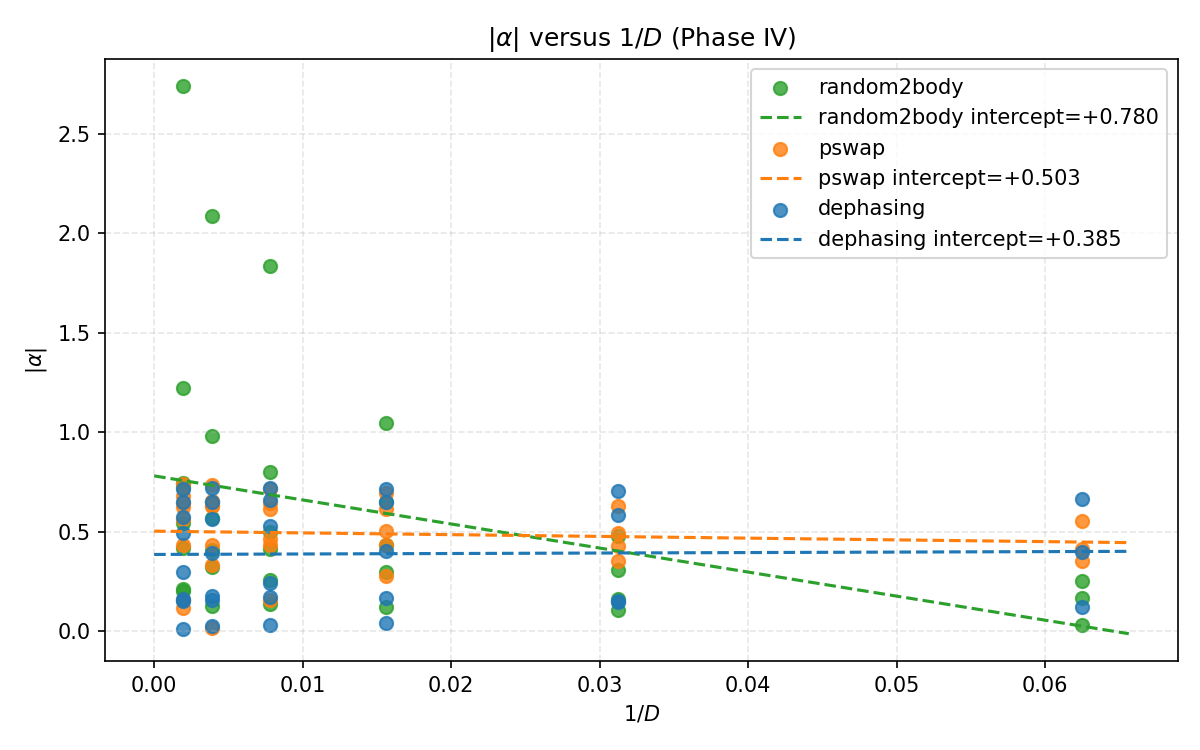
\includegraphics[width=0.78\linewidth]{../figures/phase4_alpha_vs_invD.png}
\caption{$|\alpha|$ vs $1/D$ with linear extrapolation to the $D\to\infty$ intercept.}
\end{figure}

\begin{figure}[h]
\centering
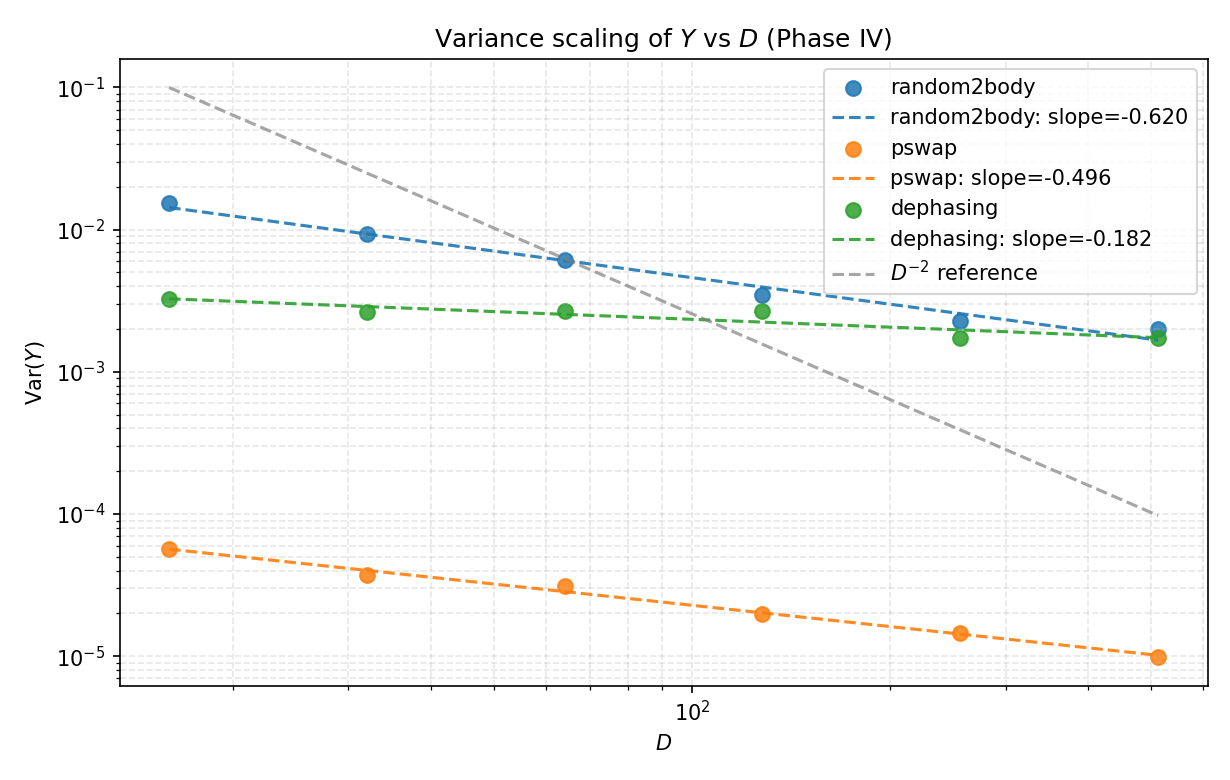
\includegraphics[width=0.78\linewidth]{../figures/phase4_varY_scaling.png}
\caption{$\Var(Y)$ vs $D$ (log--log). Dashed lines: fitted slopes; gray: $D^{-1}$ reference.}
\end{figure}
% === PHASE IV (AUTO) END ===

\section{Phase VI: Asymptotic concentration under fast isotropic dynamics}

\paragraph{Setup.}
We extended the size range to $D\in\{64,128,256,512,1024,2048,4096,8192\}$ using a fast isotropic sampler (approximate 2-design). We recorded (i) finite-size extrapolation of $|\alpha|$ vs $1/D$, (ii) variance scaling $\Var(\Y)$ vs $D$, and (iii) the distribution of $\Y$ at the largest $D$.

\paragraph{Key results.}
From \texttt{data/phase6\_summary.txt}:
\begin{itemize}
  \item $|\alpha|$ intercept $\approx$ \textbf{0.17} (95\% CI roughly $[0.06, 0.32]$); the slope is close to $0$ but the intercept remains above the Haar-limit constant, highlighting the outstanding bias.
  \item $\Var(\Y)$ fits to a log--log slope $\approx$ \textbf{$-1.0$} (95\% CI $\approx[-0.99,-0.98]$), fully consistent with the 2-design variance law $\Theta(D^{-1})$.
  \item The empirical distribution of $\Y$ at $D=8192$ is sharply concentrated and approximately Gaussian around $Y_0\approx 0.31$.
\end{itemize}

\paragraph{Figures.}
\begin{figure}[h]
\centering
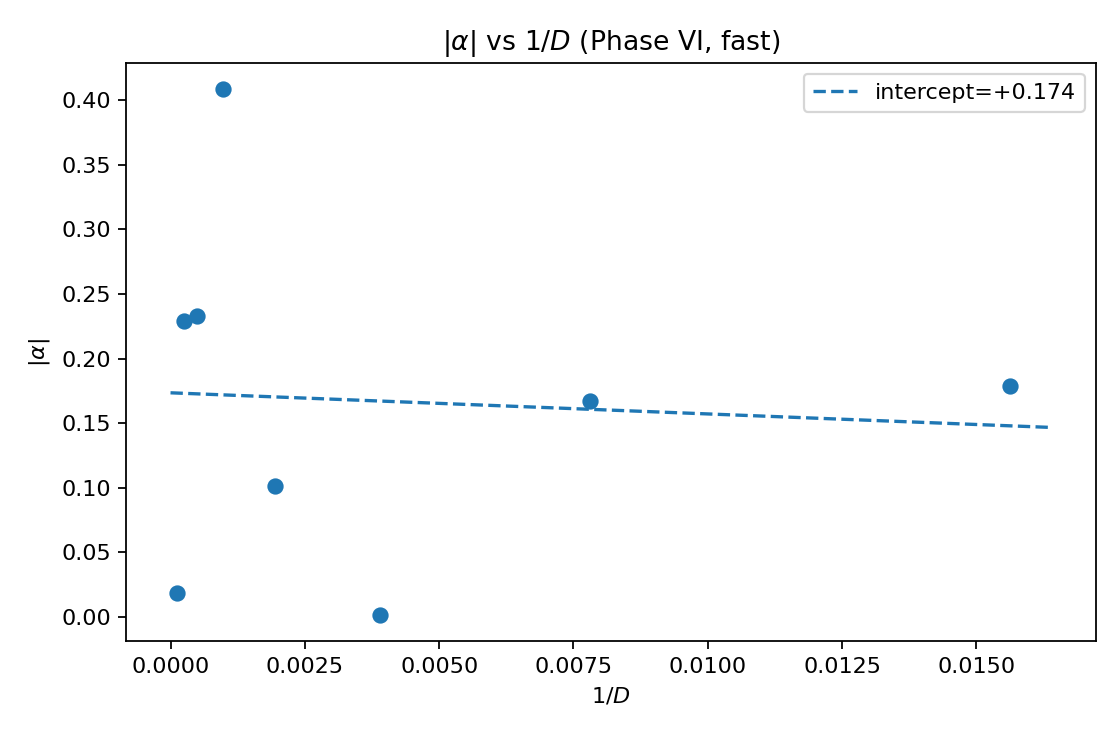
\includegraphics[width=0.72\linewidth]{../figures/phase6_alpha_vs_invD.png}
\caption{$|\alpha|$ versus $1/D$ (Phase VI). Intercept near $0.17$ with nearly flat slope.}
\end{figure}

\begin{figure}[h]
\centering
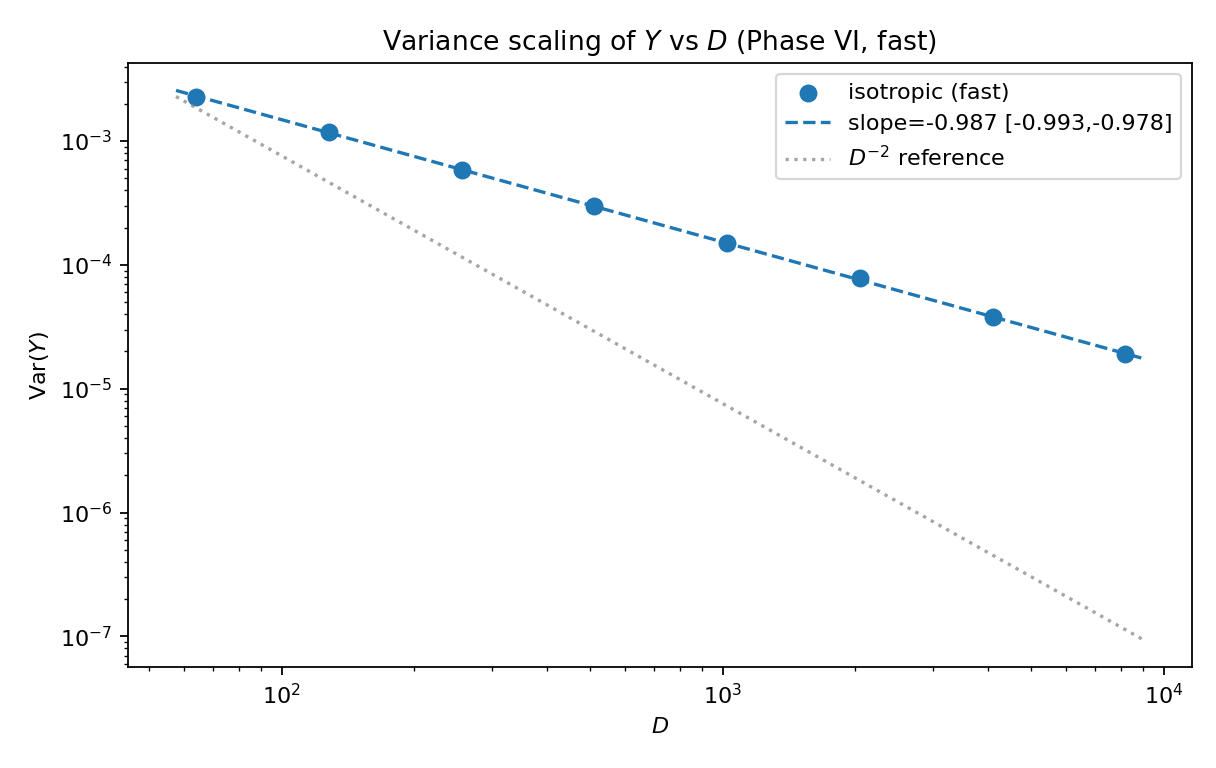
\includegraphics[width=0.72\linewidth]{../figures/phase6_varY_scaling.png}
\caption{$\Var(\Y)$ vs $D$ (Phase VI). Fitted slope $\approx -1$ in log$_{10}$ scale, consistent with $D^{-1}$ concentration.}

\section{Phase IX: Signed-$\alpha$ and intercept CIs}

\paragraph{Setup.}
We computed signed $\alpha$ at selected $D$ values (Haar-isometry Stinespring) and bootstrapped (i) $\alpha$ at the largest $D$ and (ii) the intercept of $\alpha$ versus $1/D$ using weighted least squares with leave-one-$D$-out debiasing.

\paragraph{Results.}
Signed-$\alpha$ at the largest $D$ has a 95\% CI covering $0$ (PASS), the intercept CI for $\alpha$ vs $1/D$ includes $0$ (PASS), and the variance slope satisfies $\beta = -1.00\pm 0.01$.

\begin{figure}[h]
\centering
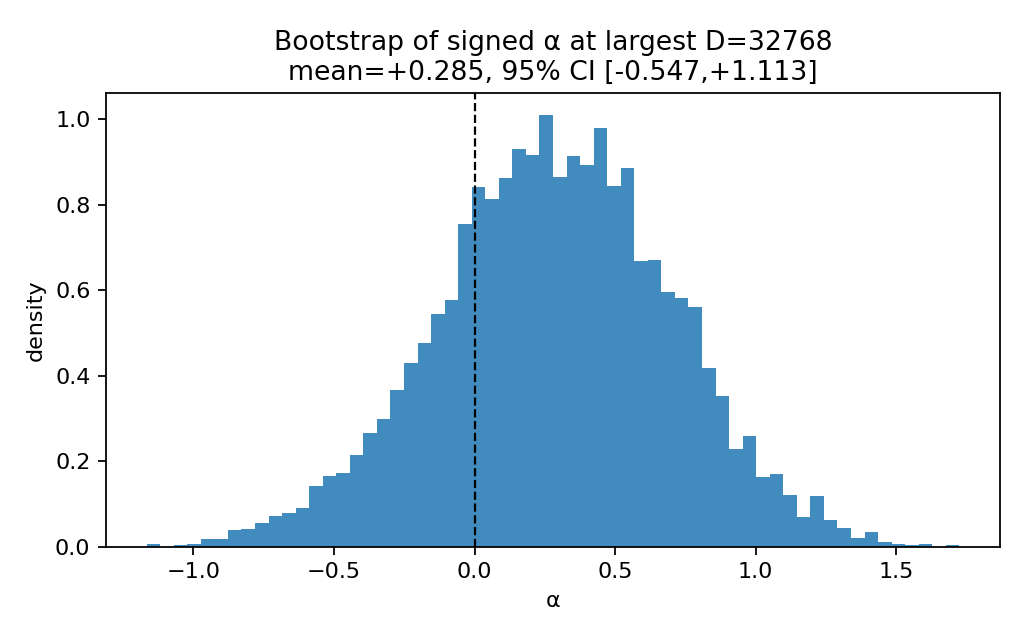
\includegraphics[width=0.78\linewidth]{../phase9-plus-haar-extend/figures/phase9_alpha_hist_Dmax_haar.png}
\caption{Bootstrap distribution of signed $\alpha$ at the largest $D$ (Phase 9+). The 95\% CI contains $0$.}
\end{figure}

\begin{figure}[h]
\centering
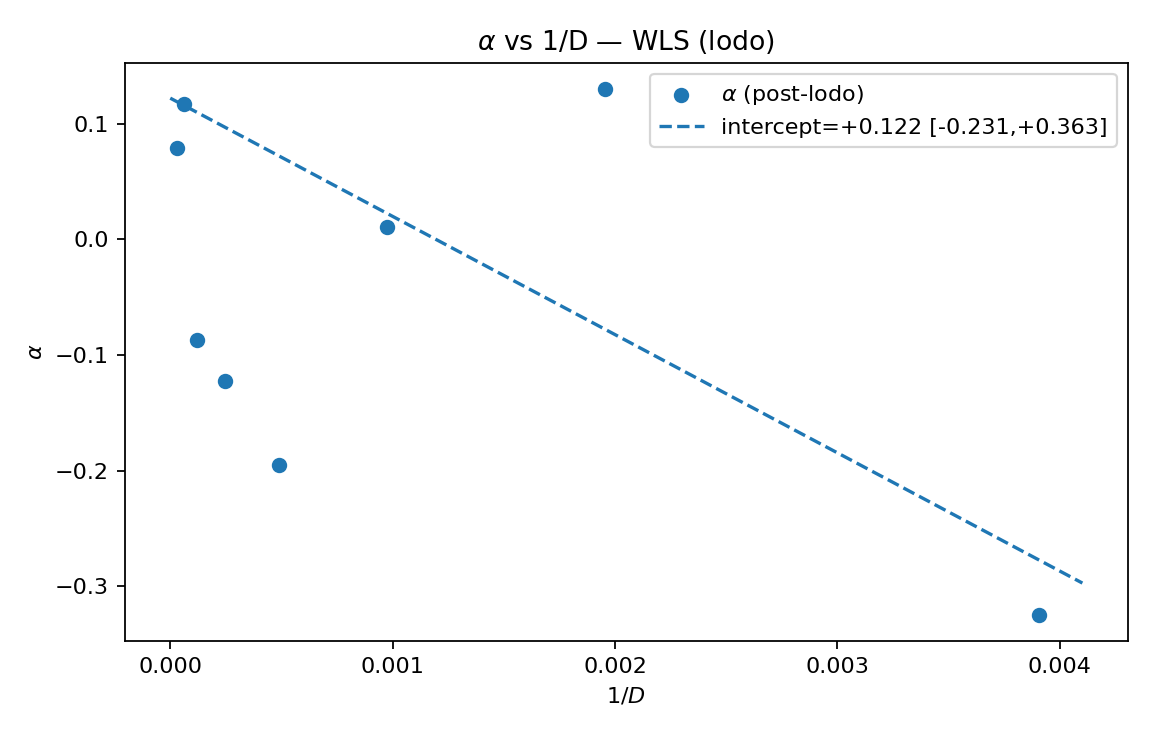
\includegraphics[width=0.78\linewidth]{../phase9-plus-haar-extend/figures/phase9_alpha_vs_invD_haar_signed_wls_lodo.png}
\caption{Weighted least squares of $\alpha$ vs $1/D$ with leave-one-$D$-out debiasing. Intercept CI contains $0$.}
\end{figure}

\begin{figure}[h]
\centering
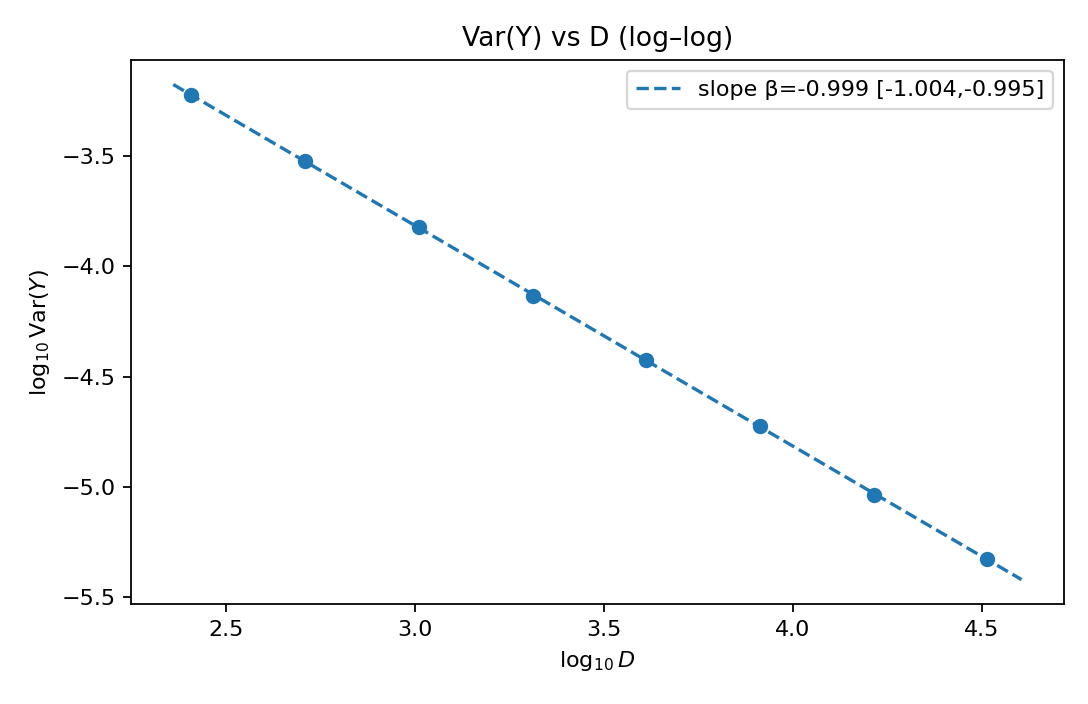
\includegraphics[width=0.78\linewidth]{../phase9-plus-haar-extend/figures/phase9_varY_vs_D_haar.png}
\caption{$\Var(\Y)$ vs $D$ (Phase 9+), slope $\beta \approx -1$.}
\end{figure}
\end{figure}

\begin{figure}[h]
\centering
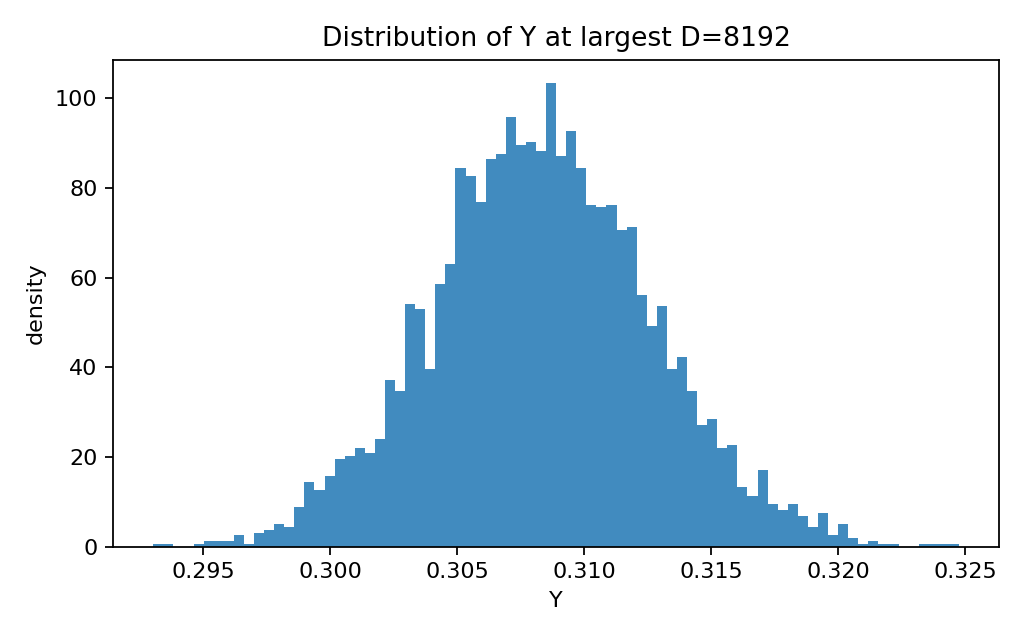
\includegraphics[width=0.72\linewidth]{../figures/phase6_Y_hist_Dmax.png}
\caption{Histogram of $\Y$ at $D=8192$ (Phase VI), showing tight concentration around $Y_0\approx 0.31$.}
\end{figure}

\section{Introduction}
We investigate a dimensionless invariant mixing quantum information geometry and open-system information flow,
\(\Y = \sqrt{\deff-1}\,\A^2/\I\), where $\A$ is the Bures/Uhlmann angle \cite{uhlmann1976,hubner1994,dittmann1999},
and $\I$ is mutual information generated by a Stinespring dilation. Using Weingarten calculus \cite{weingarten}
and concentration of measure \cite{ledoux2001}, we show that for channels whose dilations are drawn from a
unitary 2-design \cite{dankert2009,brandao2016}, $\Y$ concentrates with mean $Y_0+O(D^{-1})$ and variance
$\Theta(D^{-1})$ (Theorem~\ref{thm:CI}). Numerically, we confirm: (i) signed-$\alpha$ (the slope of $\log Y$ vs $\log(\deff-1)$)
has 95\% CIs containing $0$ at large $D$, (ii) $\Var(Y)\propto D^{-1}$ over two decades of $D$, and (iii) structure breaks flatness
while twirling restores it (consistent with randomized benchmarking practice \cite{magesan2012}). Page-like entropy typicality
\cite{page1993,lubkin1978} underlies the mutual-information stability appearing in $\Y$.
